\documentclass[a4paper,10pt,onecolumn]{IEEEtran}
\usepackage{iftex}
\ifPDFTeX
  \usepackage[T1]{fontenc}
  \usepackage[utf8]{inputenc}
\else
  \usepackage{fontspec}
  \setmainfont{texgyretermes}[Extension=.otf,
    UprightFont=*-regular, BoldFont=*-bold,
    ItalicFont=*-italic, BoldItalicFont=*-bolditalic]
  \setmonofont{texgyrecursor}[Extension=.otf,
    UprightFont=*-regular, BoldFont=*-bold,
    ItalicFont=*-italic, BoldItalicFont=*-bolditalic]
\fi
\usepackage{amsmath,amssymb,booktabs,graphicx,cite}
\usepackage[hyphens]{url}
\usepackage[hidelinks]{hyperref}
\newcommand{\repositorylink}{\url{https://github.com/ada-teodorescu/forecastability-limits-proxy-bciaut-p300}}
\ExplSyntaxOn
\cs_set_protected:Npn \path #1
  {
    \texttt{\str_map_inline:nn {#1}
      {##1 \str_case:nnF {##1}
        {{_}{\allowbreak} {/}{\allowbreak} {.}{\allowbreak} {-}{\allowbreak}}
        {\penalty500}}}
  }
\ExplSyntaxOff
\renewcommand{\thetable}{S\arabic{table}}
\renewcommand{\thefigure}{S\arabic{figure}}
\renewcommand{\theequation}{S\arabic{equation}}
\setlength{\parskip}{3pt}
\setlength{\parindent}{0pt}
\pagestyle{plain}
\title{Supplementary Methods and Results\\[4pt]
\large Forecastability Limits of a P300-Derived EEG Proxy in BCIAUT-P300}
\author{Ada Daniela Teodorescu and Alin Brîndușescu}
\begin{document}
\maketitle
\thispagestyle{plain}
\textit{Original analysis snapshot: 8 October 2026; additional diagnostics and presentation: 11 October 2026.}

These companion materials are separate from the six-page conference
manuscript.

These materials expose all 17 evaluated variants, the original tested contrasts,
subject-level differences, ranking aggregation, and existing robustness runs.
The original 5--25-block benchmark uses saved predictions and subject-fold
metrics without retraining. An additional five-model analysis at horizons
1--4 fitted learned models anew and added 32 direct context-mean comparisons.
Its results and inference family are reported separately. The supplement
generator reads these completed outputs and fits only the new affine calibration
correction described in Section~\ref{sec:supp_calibration_correction}. Bootstrap intervals
are descriptive and unadjusted.

\section{Exact proxy construction and annotation requirements}

Each preprocessed epoch has eight channels and 128 time samples.
The target and non-target prototypes $P_{\mathrm T}$ and $P_{\mathrm{NT}}$
average their corresponding epochs in avatar-cued calibration blocks 10--19.
Let $\bar E_b$ average the task-designated target epochs in block $b$.
The augmented representation is
\begin{equation}
X_b=[P_{\mathrm T};P_{\mathrm{NT}};\bar E_b],
\qquad \widetilde C_b=\operatorname{OAS}(X_b^\top).
\end{equation}
This is a $24\times128$ matrix; semicolons denote vertical concatenation.
OAS treats the 128 time points
as observations and 24 augmented channels as variables; it estimates and
removes each variable's temporal mean
(\texttt{assume\_centered=False}) \cite{ChenWienerShrinkage2010}.
This specifies the estimator's input convention; it does not imply
independent ERP time samples.

The unaligned score references are
\begin{equation}
R_{\mathrm T}=\operatorname{OAS}([P_{\mathrm T};P_{\mathrm{NT}};P_{\mathrm T}]^\top),
\qquad
R_{\mathrm{NT}}=\operatorname{OAS}([P_{\mathrm T};P_{\mathrm{NT}};P_{\mathrm{NT}}]^\top).
\end{equation}
They substitute each calibration prototype for the block response.
These deterministic endpoints occupy the same augmented space as $X_b$
and define a prototype-proximity margin without estimating references
from future online blocks. They are not empirical Riemannian class means.
The augmented ERP representation is inspired by Barachant and Congedo
\cite{Barachant2014}; their decoding method does not independently validate
this duplicated-prototype, block-averaged proxy.

The affine-invariant distance and session calibration mean are
\begin{equation}
d_R(A,B)=\|\log(A^{-1/2}BA^{-1/2})\|_F,\qquad
G=\arg\min_{G\succ0}\sum_{j=0}^{19}d_R^2(G,\widetilde C_j).
\end{equation}
All 20 calibration blocks enter $G$ \cite{Moakher2005}.
For $W=G^{-1/2}$, the aligned block covariance is
$C_b=W\widetilde C_bW^\top$ and aligned references are
$C_k^{\mathrm{ref}}=WR_kW^\top$, for $k\in\{\mathrm T,\mathrm{NT}\}$.
The score is
$s_b=d_R(C_b,C_{\mathrm{NT}}^{\mathrm{ref}})
      -d_R(C_b,C_{\mathrm T}^{\mathrm{ref}})$.
The tangent matrix is $\log(C_b)$, vectorized in row-wise upper-triangle
order with off-diagonal entries multiplied by $\sqrt2$ and diagonal entries
unchanged, yielding 300 features.

For the same invertible $W$,
$d_R(WAW^\top,WBW^\top)=d_R(A,B)$ \cite{Congedo2017}.
Whitening prepares tangent features for modelling; it does not itself
remove session variation from the scalar margin. Session-specific
prototypes, reference geometry, calibration fit, and averaging precision
can contribute to the score's scale and stability.

The analysis uses released target annotations retrospectively. An avatar-task
controller can know the instructed target and each flashed object's identity.
Prospective computation requires synchronized cue/stimulus metadata.
The instructed target does not establish actual participant attention.
The original adaptive ERP method also discusses supervised online target
metadata \cite{Barachant2014}. Attention or engagement interpretation
requires independent behavioural validation.

\clearpage
\section{Training, inference, and descriptive diagnostics}

\subsection{Training settings and existing robustness runs}

The main GRUs have one recurrent layer and Gaussian mean/scale outputs.
Hidden dimension is selected from $\{32,64\}$ and learning rate from
$\{10^{-3},5\times10^{-4}\}$; dropout is 0.2 and weight decay is $10^{-4}$.
EEG-containing GRUs use 20 PCA components fitted on current training subjects.
Batch size is 64, the optimizer is Adam, and the main benchmark uses at most
200 epochs with early-stopping patience 20 and no gradient clipping.
The short-horizon analysis uses the same historical point-forecasting
implementation, preserved in commit \texttt{48de5b0} and included as
\path{src/experiments/exp41_historical_step8.py}.
Selection minimizes validation Gaussian NLL, while the primary point metric
is MAE; these runs do not exhaust GRUs selected to optimize MAE.

The portable repository's \path{pipeline/reproduce_paper_gru.py} command
restores these historical stopping settings and disables gradient clipping
for the main and robustness comparisons. The general Step 8 entrypoint
retains later defaults of 100 epochs, patience 10, and gradient clipping;
it is not the paper-training command. Validation training and final refitting
are compared with the preserved historical implementation in synthetic tests.

The last two outer-training subjects by sorted identifier provide main
inner validation. A fresh model is refitted on all 14 training subjects
for the best validation epoch. That validation pair is repeated in most
outer folds. Archived \texttt{exp30} instead uses five-fold inner
GroupKFold by subject, selecting by validation-size-weighted mean best NLL.
It refits for the rounded mean of the selected candidate's five best epochs,
with a minimum of one. Archived \texttt{exp31} uses the same grouped protocol
and adds dropout $\{0,0.2\}$, yielding eight hyperparameter combinations.

Tasks are enumerated by horizon, target view, ablation, and held-out subject.
For zero-based task index $i$, candidate $g$ on inner split $j$ uses seed
$20260330+101i+g\,n_{\mathrm{inner}}+j$; final refitting uses
$20260330+101i+97$. PyTorch and the shuffled DataLoader use these seeds.
Deterministic algorithms are requested with \texttt{warn\_only=True};
cross-platform bitwise reproducibility is not asserted.
Model-selection CSVs record selected settings and refit epochs.

\subsection{Point metrics, original contrasts, and intervals}

For held-out subject $u$ at horizon $h$, mean absolute error is
\begin{equation}
\mathrm{MAE}_{u,h}
=\frac{1}{n_{u,h}}\sum_{i=1}^{n_{u,h}}|y_i-\hat y_i|,
\end{equation}
where $y_i$ is the observed target, $\hat y_i$ is its prediction, and
$n_{u,h}$ is the number of valid forecasting examples.
Reported MAE averages these 15 subject values with equal weights.
For anchor block $b$, the context mean is
$m_b=\frac{1}{10}\sum_{j=0}^{9}s_{b-j}$.
Residual fitting uses $r_{b,h}=s_{b+h}-m_b$; adding $m_b$ to a residual
forecast reconstructs the raw-score forecast without changing its
absolute error.

Seven classical and ten GRU contrasts are listed in
Tables~\ref{tab:supp_contrasts_classical}--\ref{tab:supp_contrasts_gru}.
Each is evaluated for MAE and Gaussian NLL, both views, and five horizons:
$(7+10)\times2\times2\times5=340$ comparisons.
Holm correction \cite{Holm1979} applies separately within each horizon,
view, metric, and classical/GRU family: 40 correction families.
These are selected contrasts, not exhaustive direct baseline comparisons.
The archived CSV retains zero-handling, p-value method, effects,
original bootstrap intervals, and adjusted p-values.
Three GRU templates use the best of nine trained classical candidates,
selected separately by the lowest aggregate outer-subject mean of the
tested metric (ties use the other metric, then model name). That
post-hoc comparator selection makes those contrasts exploratory.
The 20 horizon/view/metric selections are exposed in a separate CSV;
the 17 templates instantiate 23 distinct ordered model pairs.
Signed-rank interpretation assumes independent subject differences with
approximately symmetric distributions; shared LOSO training makes
independence an approximation.

New 95\% intervals resample paired subject differences or subject ranking
aggregates 10,000 times, with NumPy seed 20261007, using the 2.5th and 97.5th
percentiles of the mean. They are descriptive, unadjusted intervals,
not new tests or simultaneous intervals. They condition on fitted predictions,
omit repeated-training/model-selection uncertainty, and inherit the shared-fold
independence limitation. For the main benchmark, formal statements use only
the original contrasts; the additional fixed-baseline tests below form a separate
post-hoc family.

The main paper's paired-$t$ approximation estimates the mean MAE improvement
detectable with approximately 80\% power in a two-sided, uncorrected test at
$\alpha=0.05$. It uses the observed standard deviation of the 15 subject-fold
differences and assumes independent, approximately normal differences.
Shared LOSO training makes independence an approximation.
For the raw score-only GRU versus context mean, $\delta_{80}$ is approximately
0.0040 at horizons 5 and 10 and 0.0087 at horizon 25
(2.3--4.9\% of baseline MAE).
These values are rough sensitivity estimates, not power calculations for
the Holm-corrected signed-rank analysis or evidence against smaller gains.

\clearpage
\subsection{Ranking aggregation and probabilistic scores}

Let $\tau$ be 80\% of the session's avatar-cued calibration mean.
All 105 means are positive: minimum 1.279, first quartile 2.022,
median 2.293, third quartile 2.479, maximum 3.280. Thus the signed-margin
threshold has no nonpositive or near-zero calibration references in this sample.
The underlying score remains signed and unvalidated behaviourally.
The avatar-cued blocks also contribute to the prototypes, so this is an
in-sample calibration reference, not an independently validated threshold.
It uses no future online blocks; a cross-fitted calibration threshold remains
an untested sensitivity analysis.
The low-proxy endpoint and its Gaussian forecast probability are
\begin{equation}
D_{b,h}=\mathbf{1}\{s_{b+h}<\tau\},\qquad
p(D_{b,h}=1)=\Phi\!\left(\frac{\tau-\mu_{\mathrm{raw}}}{\sigma}\right),
\end{equation}
where $\Phi$ is the standard normal cumulative distribution function
and $\sigma$ is the forecast standard deviation. Raw-score and residual
GRUs are fitted separately, with
\begin{equation}
\mu_{\mathrm{raw}}=
\begin{cases}
\hat\mu, & \text{raw-score fit},\\
m_b+\hat\mu_r, & \text{residual fit}.
\end{cases}
\end{equation}
Each fit learns its own $\sigma$. In residual coordinates, the same event
is $r_{b,h}<\tau-m_b$, so the endpoint labels do not change.
The context-mean comparator has $\mu_{\mathrm{raw}}=m_b$ in both views
and the same training-fold residual standard deviation for $\sigma$.
Matching predictions by subject, session, horizon, and block therefore
gives identical comparator probabilities up to numerical precision.

Pooled ROC-AUC combines all eligible examples from a held-out subject's seven
sessions, then gives subjects equal weight. Positive--negative pairs from
different sessions contribute. Average precision uses the scikit-learn
average-precision function, rather than trapezoidal integration.
The session-restricted diagnostic computes ROC-AUC and average precision
in sessions with both endpoint classes, averages sessions within subjects,
then averages subjects. At horizon 5, 103 sessions are eligible; two have
no low-proxy examples. All 15 subjects retain eligible sessions.
Both predictors and both metrics use the same eligible-session set.
No new significance test is supplied. Intervals resample subject aggregates
and describe a different estimand from pooled AUC.

Gaussian NLL is
$\frac12\log(2\pi)+\log\sigma+(y-\mu)^2/(2\sigma^2)$ (lower is better);
a density-based NLL can be negative.
Nominal 80\% Gaussian width is $2\Phi^{-1}(0.9)\sigma$.
NLL, width, and coverage are averaged within subjects, then across subjects.
Coverage alone establishes neither conditional calibration nor sharpness.

\subsection{Variance decomposition and block horizons}

For balanced scores $x_{ujb}$ from 15 subjects, seven sessions, and 50 blocks,
let $\bar x_u$, $\bar x_{uj}$, and $\bar x$ be subject, session, and grand means.
The descriptive population-variance partition is
\begin{align}
V_{\mathrm{sub}}&=\frac1{15}\sum_u(\bar x_u-\bar x)^2,\\
V_{\mathrm{sess}}&=\frac1{105}\sum_{u,j}(\bar x_{uj}-\bar x_u)^2,\\
V_{\mathrm{within}}&=\frac1{5250}\sum_{u,j,b}(x_{ujb}-\bar x_{uj})^2.
\end{align}
These sum to empirical population variance (denominator $N$, not $N-1$);
they are not fitted random-effects components.
The full-session mean includes future observations and is only a retrospective
diagnostic. Its context-mean correlation partly reflects shared observations.

Block units align forecasts with completed task blocks.
Eight 100 ms flashes with 200 ms gaps give $2.4K$ seconds of stimulation
per block, for $K\in[3,10]$. Ignoring cue, feedback, and pauses, five blocks
span 36--120 seconds of stimulation. Five evenly spaced offsets, 5 through
25 blocks, were selected to compare increasingly distant forecasts.
This is a benchmark grid, not an intervention-latency or clinical prescription.
The additional five-model analysis evaluates horizons 1--4 separately.

\clearpage
\section{Complete model results}

Tables~\ref{tab:supp_mae_raw} and \ref{tab:supp_mae_residual} show all 17 variants,
with equal-subject mean MAE. The lowest residual mean can differ from the
context mean without establishing a reliable improvement in a tested contrast.
Residual \emph{EEG-only} denotes the learned correction's inputs; reconstructing
a raw forecast still adds the score context mean.
The companion CSV includes subject SDs, RMSE, paired differences,
and original direct-baseline-test status.

\begin{table}[!ht]
\centering
\small
\setlength{\tabcolsep}{5pt}
\renewcommand{\arraystretch}{1.1}
\caption{All 17 raw-score variants. Equal-subject mean MAE; bold denotes the lowest descriptive mean, not a significance claim.}
\label{tab:supp_mae_raw}
\begin{tabular}{lrrrrr}
\toprule
Model & 5 & 10 & 15 & 20 & 25 \\
\midrule
Context mean & \textbf{0.1746} & \textbf{0.1741} & \textbf{0.1767} & \textbf{0.1773} & \textbf{0.1752} \\
Persistence & 0.2320 & 0.2256 & 0.2318 & 0.2400 & 0.2414 \\
Moving average (5) & 0.1829 & 0.1824 & 0.1829 & 0.1868 & 0.1869 \\
Training mean & 0.3431 & 0.3435 & 0.3427 & 0.3403 & 0.3383 \\
AR ridge (5) & 0.1828 & 0.1816 & 0.1827 & 0.1860 & 0.1852 \\
GRU score & 0.1780 & 0.1772 & 0.1814 & 0.1815 & 0.1809 \\
\midrule
EEG ridge & 0.3656 & 0.3633 & 0.3607 & 0.3552 & 0.3527 \\
EEG elastic-net & 0.3406 & 0.3400 & 0.3378 & 0.3352 & 0.3325 \\
EEG PCR & 0.3423 & 0.3439 & 0.3432 & 0.3394 & 0.3365 \\
EEG PLS & 0.3579 & 0.3582 & 0.3587 & 0.3538 & 0.3532 \\
Riemannian KNN & 0.3783 & 0.3749 & 0.3676 & 0.3743 & 0.3611 \\
GRU EEG & 0.3365 & 0.3378 & 0.3332 & 0.3258 & 0.3404 \\
Permuted EEG PCR & 0.3423 & 0.3439 & 0.3428 & 0.3396 & 0.3365 \\
\midrule
Hybrid ridge & 0.1895 & 0.1878 & 0.1933 & 0.1953 & 0.1943 \\
Hybrid PCR & 0.2970 & 0.2954 & 0.2972 & 0.2990 & 0.3020 \\
Hybrid PLS & 0.2561 & 0.2601 & 0.2672 & 0.2622 & 0.2695 \\
GRU hybrid & 0.1922 & 0.1938 & 0.1924 & 0.1930 & 0.1898 \\
\bottomrule
\end{tabular}
\end{table}

\begin{table}[!ht]
\centering
\small
\setlength{\tabcolsep}{5pt}
\renewcommand{\arraystretch}{1.1}
\caption{All 17 separately fitted residual-target variants. Equal-subject mean MAE; bold denotes the lowest descriptive mean, not a significance claim.}
\label{tab:supp_mae_residual}
\begin{tabular}{lrrrrr}
\toprule
Model & 5 & 10 & 15 & 20 & 25 \\
\midrule
Context mean & 0.1746 & 0.1741 & \textbf{0.1767} & 0.1773 & 0.1752 \\
Persistence & 0.2320 & 0.2256 & 0.2318 & 0.2400 & 0.2414 \\
Moving average (5) & 0.1829 & 0.1824 & 0.1829 & 0.1868 & 0.1869 \\
Training mean & 0.1748 & 0.1745 & 0.1772 & 0.1776 & 0.1752 \\
AR ridge (5) & 0.1747 & 0.1740 & 0.1771 & \textbf{0.1769} & 0.1747 \\
GRU score & 0.1752 & 0.1743 & 0.1775 & 0.1777 & 0.1753 \\
\midrule
EEG ridge & 0.1792 & 0.1787 & 0.1822 & 0.1844 & 0.1770 \\
EEG elastic-net & 0.1747 & 0.1745 & 0.1772 & 0.1772 & \textbf{0.1747} \\
EEG PCR & 0.1747 & 0.1737 & 0.1785 & 0.1787 & 0.1759 \\
EEG PLS & 0.1800 & 0.1802 & 0.1823 & 0.1829 & 0.1856 \\
Riemannian KNN & 0.1911 & 0.1937 & 0.1929 & 0.1944 & 0.1924 \\
GRU EEG & 0.1744 & 0.1744 & 0.1789 & 0.1798 & 0.1775 \\
Permuted EEG PCR & 0.1751 & 0.1746 & 0.1775 & 0.1790 & 0.1759 \\
\midrule
Hybrid ridge & 0.1780 & 0.1777 & 0.1823 & 0.1818 & 0.1765 \\
Hybrid PCR & 0.1743 & \textbf{0.1735} & 0.1782 & 0.1791 & 0.1760 \\
Hybrid PLS & 0.1796 & 0.1797 & 0.1820 & 0.1820 & 0.1847 \\
GRU hybrid & \textbf{0.1737} & 0.1744 & 0.1782 & 0.1782 & 0.1762 \\
\bottomrule
\end{tabular}
\end{table}


\clearpage
\section{Paired differences from the primary comparator}

Positive differences mean worse MAE than the context mean; negative values
mean lower descriptive MAE. Tables~\ref{tab:supp_deltas_raw} and
\ref{tab:supp_deltas_residual} show horizons 5 and 25.
All five horizons and individual subject differences are in the CSVs.
A dash in the final column means that direct comparison was outside the
original contrast family. No significance decision is inferred from the
unadjusted intervals. The companion paired-difference plot in the release
package uses the same interval procedure. Main-paper Figure 5 contrasts
retrospective lag correlations with raw- and residual-target GRU MAE
differences and these descriptive intervals.

\begin{table}[!ht]
\centering
\small
\setlength{\tabcolsep}{5pt}
\renewcommand{\arraystretch}{1.1}
\caption{Raw-target MAE differences (model minus context mean), with unadjusted descriptive 95\% subject-fold bootstrap intervals. The final column identifies an original direct baseline test.}
\label{tab:supp_deltas_raw}
\begin{tabular}{lrrr}
\toprule
Model & $h=5$: difference [CI] & $h=25$: difference [CI] & Direct test \\
\midrule
Persistence & +0.0575 [+0.0492, +0.0651] & +0.0662 [+0.0595, +0.0725] & Yes \\
Moving average (5) & +0.0084 [+0.0062, +0.0104] & +0.0117 [+0.0086, +0.0147] & -- \\
Training mean & +0.1686 [+0.1199, +0.2221] & +0.1631 [+0.1165, +0.2134] & -- \\
AR ridge (5) & +0.0082 [+0.0057, +0.0109] & +0.0099 [+0.0065, +0.0135] & -- \\
GRU score & +0.0034 [+0.0011, +0.0062] & +0.0057 [+0.0003, +0.0113] & Yes \\
EEG ridge & +0.1911 [+0.1483, +0.2400] & +0.1775 [+0.1372, +0.2243] & -- \\
EEG elastic-net & +0.1660 [+0.1199, +0.2171] & +0.1573 [+0.1151, +0.2032] & -- \\
EEG PCR & +0.1677 [+0.1203, +0.2208] & +0.1613 [+0.1183, +0.2069] & Yes \\
EEG PLS & +0.1833 [+0.1375, +0.2370] & +0.1779 [+0.1338, +0.2279] & -- \\
Riemannian KNN & +0.2037 [+0.1731, +0.2335] & +0.1858 [+0.1528, +0.2175] & -- \\
GRU EEG & +0.1620 [+0.1251, +0.2077] & +0.1651 [+0.1272, +0.2113] & Yes \\
Permuted EEG PCR & +0.1678 [+0.1205, +0.2208] & +0.1613 [+0.1184, +0.2068] & -- \\
Hybrid ridge & +0.0150 [+0.0095, +0.0216] & +0.0191 [+0.0148, +0.0233] & Yes \\
Hybrid PCR & +0.1224 [+0.0931, +0.1602] & +0.1268 [+0.0970, +0.1618] & Yes \\
Hybrid PLS & +0.0815 [+0.0638, +0.1054] & +0.0942 [+0.0765, +0.1139] & -- \\
GRU hybrid & +0.0177 [+0.0071, +0.0315] & +0.0145 [+0.0058, +0.0242] & Yes \\
\bottomrule
\end{tabular}
\end{table}

\begin{table}[!ht]
\centering
\small
\setlength{\tabcolsep}{5pt}
\renewcommand{\arraystretch}{1.1}
\caption{Residual-target MAE differences (model minus context mean), with unadjusted descriptive 95\% subject-fold bootstrap intervals. The final column identifies an original direct baseline test.}
\label{tab:supp_deltas_residual}
\begin{tabular}{lrrr}
\toprule
Model & $h=5$: difference [CI] & $h=25$: difference [CI] & Direct test \\
\midrule
Persistence & +0.0575 [+0.0492, +0.0651] & +0.0662 [+0.0595, +0.0725] & Yes \\
Moving average (5) & +0.0084 [+0.0062, +0.0104] & +0.0117 [+0.0086, +0.0147] & -- \\
Training mean & +0.0003 [+0.0001, +0.0005] & -0.0000 [-0.0012, +0.0012] & -- \\
AR ridge (5) & +0.0002 [-0.0002, +0.0005] & -0.0005 [-0.0018, +0.0009] & -- \\
GRU score & +0.0006 [-0.0002, +0.0015] & +0.0001 [-0.0012, +0.0014] & Yes \\
EEG ridge & +0.0047 [+0.0030, +0.0068] & +0.0018 [-0.0009, +0.0047] & -- \\
EEG elastic-net & +0.0001 [-0.0002, +0.0005] & -0.0005 [-0.0025, +0.0014] & -- \\
EEG PCR & +0.0002 [-0.0012, +0.0019] & +0.0007 [-0.0007, +0.0023] & Yes \\
EEG PLS & +0.0055 [+0.0016, +0.0098] & +0.0104 [+0.0056, +0.0153] & -- \\
Riemannian KNN & +0.0165 [+0.0130, +0.0203] & +0.0171 [+0.0126, +0.0219] & -- \\
GRU EEG & -0.0001 [-0.0015, +0.0012] & +0.0023 [-0.0011, +0.0062] & Yes \\
Permuted EEG PCR & +0.0005 [+0.0002, +0.0009] & +0.0007 [-0.0008, +0.0024] & -- \\
Hybrid ridge & +0.0035 [+0.0020, +0.0049] & +0.0013 [-0.0013, +0.0042] & Yes \\
Hybrid PCR & -0.0002 [-0.0017, +0.0015] & +0.0008 [-0.0007, +0.0023] & Yes \\
Hybrid PLS & +0.0051 [+0.0012, +0.0096] & +0.0095 [+0.0049, +0.0143] & -- \\
GRU hybrid & -0.0009 [-0.0023, +0.0005] & +0.0009 [-0.0012, +0.0033] & Yes \\
\bottomrule
\end{tabular}
\end{table}


\clearpage
\section{Exact original contrast families}

Each family is repeated for every horizon, target view, and metric.
Archived differences use model B minus model A; the preceding paired tables
consistently use alternative minus context mean.
All 340 original tests are preserved in \path{original_tested_contrasts.csv}.
In the GRU table, the selected trained comparator is AR ridge (5) for all
raw-view comparisons and all Gaussian-NLL comparisons. For residual MAE,
it is hybrid PCR at horizons 5 and 10, AR ridge (5) at 15 and 20, and EEG
elastic-net at 25. The selection CSV gives every metric-specific instance.

\begin{table}[!ht]
\centering
\small
\setlength{\tabcolsep}{5pt}
\renewcommand{\arraystretch}{1.1}
\caption{Original seven classical contrast templates. Archived differences use model B minus model A.}
\label{tab:supp_contrasts_classical}
\begin{tabular}{lll}
\toprule
ID & Model A & Model B \\
\midrule
C1 & Persistence & Moving average (5) \\
C2 & Context mean & Persistence \\
C3 & Context mean & Hybrid ridge \\
C4 & Context mean & EEG PCR \\
C5 & Context mean & Hybrid PCR \\
C6 & EEG PCR & Riemannian KNN \\
C7 & EEG PCR & Permuted EEG PCR \\
\bottomrule
\end{tabular}
\end{table}

\begin{table}[!ht]
\centering
\small
\setlength{\tabcolsep}{5pt}
\renewcommand{\arraystretch}{1.1}
\caption{Original ten GRU contrast templates. Archived differences use model B minus model A.}
\label{tab:supp_contrasts_gru}
\begin{tabular}{lll}
\toprule
ID & Model A & Model B \\
\midrule
G1 & GRU score & Persistence \\
G2 & GRU score & Context mean \\
G3 & GRU score & Selected trained classical \\
G4 & GRU EEG & Persistence \\
G5 & GRU EEG & Context mean \\
G6 & GRU EEG & Selected trained classical \\
G7 & GRU hybrid & Persistence \\
G8 & GRU hybrid & Context mean \\
G9 & GRU hybrid & Selected trained classical \\
G10 & GRU hybrid & GRU score \\
\bottomrule
\end{tabular}
\end{table}


\clearpage
\section{Ranking, robustness, and uncertainty}

Only session-corrected \path{review_revision/step8_anomaly_predictions.csv}
is used for ranking; historical main and robustness ranking files are excluded.
The two AUC aggregations use different pairs and session weighting.
Moderate pooled AUC does not establish within-session temporal discrimination.

\begin{table}[!ht]
\centering
\small
\setlength{\tabcolsep}{5pt}
\renewcommand{\arraystretch}{1.1}
\caption{Horizon-5 ROC-AUC, with unadjusted descriptive 95\% subject-bootstrap intervals. Session-restricted results average 103 eligible sessions within subjects, then give the 15 subjects equal weight.}
\label{tab:supp_ranking}
\begin{tabular}{llrr}
\toprule
Predictor & Fit & Sessions pooled & Within-session \\
\midrule
Context mean & Raw & 0.6353 [0.5914, 0.6821] & 0.4742 [0.4463, 0.5024] \\
GRU score & Raw & 0.6309 [0.5875, 0.6772] & 0.4692 [0.4413, 0.4967] \\
GRU EEG & Raw & 0.5010 [0.4730, 0.5307] & 0.5004 [0.4750, 0.5288] \\
GRU hybrid & Raw & 0.5984 [0.5695, 0.6284] & 0.4806 [0.4651, 0.4964] \\
Context mean & Residual & 0.6353 [0.5914, 0.6821] & 0.4742 [0.4463, 0.5024] \\
GRU score & Residual & 0.6324 [0.5893, 0.6789] & 0.4712 [0.4430, 0.4991] \\
GRU EEG & Residual & 0.6316 [0.5903, 0.6772] & 0.4781 [0.4465, 0.5069] \\
GRU hybrid & Residual & 0.6323 [0.5906, 0.6784] & 0.4798 [0.4508, 0.5077] \\
\bottomrule
\end{tabular}
\end{table}


The robustness table uses existing \texttt{exp30} and \texttt{exp31}
point-forecasting artifacts. Both raw score-only GRUs remain above the
context mean at every horizon. All GRUs, views, and horizons are included
in \path{robustness_summary.csv}.

\begin{table}[!ht]
\centering
\small
\setlength{\tabcolsep}{5pt}
\renewcommand{\arraystretch}{1.1}
\caption{Saved robustness runs: raw-target score-only GRU mean MAE.}
\label{tab:supp_robustness}
\begin{tabular}{lrrrrr}
\toprule
Protocol & 5 & 10 & 15 & 20 & 25 \\
\midrule
Context mean & 0.1746 & 0.1741 & 0.1767 & 0.1773 & 0.1752 \\
Main GRU & 0.1780 & 0.1772 & 0.1814 & 0.1815 & 0.1809 \\
Grouped inner CV & 0.1803 & 0.1783 & 0.1830 & 0.1798 & 0.1834 \\
Grouped CV + dropout search & 0.1753 & 0.1767 & 0.1783 & 0.1782 & 0.1785 \\
\bottomrule
\end{tabular}
\end{table}

\begin{table}[!ht]
\centering
\small
\setlength{\tabcolsep}{5pt}
\renewcommand{\arraystretch}{1.1}
\caption{Horizon-5 Gaussian NLL (lower is better), nominal 80\% interval coverage, and mean interval width in proxy-score units.}
\label{tab:supp_uncertainty}
\begin{tabular}{llrrr}
\toprule
Predictor & Fit & NLL & Coverage (\%) & Width \\
\midrule
Context mean & Raw & -0.0529 & 82.5 & 0.5852 \\
GRU score & Raw & -0.0702 & 84.0 & 0.6168 \\
GRU EEG & Raw & 0.6329 & 72.1 & 0.9303 \\
GRU hybrid & Raw & 0.0049 & 80.3 & 0.6184 \\
Context mean & Residual & -0.0529 & 82.5 & 0.5852 \\
GRU score & Residual & -0.0909 & 82.3 & 0.5828 \\
GRU EEG & Residual & -0.0466 & 81.6 & 0.5883 \\
GRU hybrid & Residual & -0.0721 & 81.7 & 0.5780 \\
\bottomrule
\end{tabular}
\end{table}


The main raw score-only GRU's horizon-5 NLL advantage does not establish
a reliable gain (original Holm-adjusted $p=0.4586$).
All variants' NLL, coverage, and computed Gaussian width are supplied
in \path{probabilistic_summary.csv}.

\clearpage
\section{Additional short-horizon analysis}

The five core models are the context mean, persistence, five-score AR ridge,
EEG-context PCR, and score-only GRU. The same frozen session-calibrated proxy,
ten-block history, separately fitted raw/residual targets, and 15-subject
LOSO evaluation are retained. Valid examples per subject are 280, 273, 266,
and 259 at horizons 1--4, respectively, across seven sessions.
Each horizon has its own learned coefficients, selected settings, and GRU weights.
Classical selection uses the original five-fold inner GroupKFold by subject
and MAE grids. GRU selection uses the original two-subject validation,
Gaussian NLL, four hidden-size/learning-rate candidates, 200-epoch cap,
patience 20, and best-epoch refit. The original three-ablation task enumeration
determines seed offsets, although only the score-only GRU is evaluated here.
The historical implementation reproduces the saved horizon-5 SBJ01 raw GRU
selection (64 units, learning rate 0.001, epoch 82), with maximum prediction
difference $4.77\times10^{-7}$.

PCR computes the same standardized, centred principal subspace using an exact
symmetric eigen-decomposition, with full-SVD fallback for ill-conditioned
inputs. Decompositions are shared across component candidates and target views.
Agreement with the original full-SVD estimator was verified in tests, saved
horizon-5 outputs, and three completed short-horizon subject fits, at absolute
prediction tolerance $10^{-8}$.

The four alternatives are compared directly with the context mean at each
horizon and target view, yielding 32 paired MAE tests over 15 subject values.
Two-sided Wilcoxon tests retain Pratt zero handling. Primary Holm correction
covers all 32 new comparisons; four-test correction within each horizon/view
is also reported. These are additional families, distinct from the original
seven-classical and ten-GRU families. Descriptive paired 95\% intervals use
10,000 subject bootstrap resamples with seed 20261008, condition on fitted
predictions, and omit refitting uncertainty. Shared LOSO training limits
independence. This analysis reuses the original participants and does not
constitute an independent validation cohort. No new ranking analysis is added.

Tables~\ref{tab:supp_short_mae_raw}--\ref{tab:supp_short_mae_residual} show
all five models. The context mean has the lowest raw-score mean MAE at each
short horizon. Residual EEG PCR has lower descriptive MAE at horizons 2--4;
the largest reduction is 0.000748 (0.43\%) at horizon 4, with primary
Holm-adjusted $p=0.886$. No alternative establishes a gain in either view.

\begin{table}[!ht]
\centering
\small
\setlength{\tabcolsep}{5pt}
\renewcommand{\arraystretch}{1.1}
\caption{Raw-score short-horizon MAE for the five-model extension. Values average 15 held-out subjects equally.}
\label{tab:supp_short_mae_raw}
\begin{tabular}{lrrrr}
\toprule
Model & 1 & 2 & 3 & 4 \\
\midrule
Context mean & 0.1721 & 0.1724 & 0.1736 & 0.1741 \\
Persistence & 0.2284 & 0.2298 & 0.2309 & 0.2306 \\
AR ridge (5) & 0.1793 & 0.1813 & 0.1830 & 0.1828 \\
EEG PCR & 0.3420 & 0.3433 & 0.3429 & 0.3425 \\
GRU score & 0.1736 & 0.1755 & 0.1754 & 0.1748 \\
\bottomrule
\end{tabular}
\end{table}

\begin{table}[!ht]
\centering
\small
\setlength{\tabcolsep}{5pt}
\renewcommand{\arraystretch}{1.1}
\caption{Separately fitted residual-target short-horizon MAE for the five-model extension. Values average 15 held-out subjects equally.}
\label{tab:supp_short_mae_residual}
\begin{tabular}{lrrrr}
\toprule
Model & 1 & 2 & 3 & 4 \\
\midrule
Context mean & 0.1721 & 0.1724 & 0.1736 & 0.1741 \\
Persistence & 0.2284 & 0.2298 & 0.2309 & 0.2306 \\
AR ridge (5) & 0.1723 & 0.1726 & 0.1737 & 0.1741 \\
EEG PCR & 0.1721 & 0.1723 & 0.1730 & 0.1733 \\
GRU score & 0.1730 & 0.1730 & 0.1740 & 0.1742 \\
\bottomrule
\end{tabular}
\end{table}


\clearpage
All 32 paired effects are reported below. Negative differences indicate lower
MAE than the context mean. Intervals are unadjusted and descriptive; they do
not replace the multiplicity-corrected tests or establish equivalence.

\begin{table}[!ht]
\centering
\small
\setlength{\tabcolsep}{5pt}
\renewcommand{\arraystretch}{1.1}
\caption{Raw-target short-horizon MAE differences (alternative minus context mean). Intervals are unadjusted descriptive 95\% paired-subject bootstraps. Primary $p_{32}$ corrects all 32 additional comparisons; $p_4$ corrects within each horizon/view.}
\label{tab:supp_short_pairs_raw}
\begin{tabular}{lrrlrr}
\toprule
Alternative & $h$ & $\Delta$ MAE & 95\% interval & $p_{32}$ & $p_4$ \\
\midrule
Persistence & 1 & +0.05628 & [+0.04914, +0.06454] & 0.0020 & 0.0002 \\
Persistence & 2 & +0.05740 & [+0.05207, +0.06278] & 0.0020 & 0.0002 \\
Persistence & 3 & +0.05731 & [+0.05069, +0.06372] & 0.0020 & 0.0002 \\
Persistence & 4 & +0.05655 & [+0.05080, +0.06245] & 0.0020 & 0.0002 \\
AR ridge (5) & 1 & +0.00721 & [+0.00483, +0.00945] & 0.0052 & 0.0006 \\
AR ridge (5) & 2 & +0.00885 & [+0.00648, +0.01121] & 0.0022 & 0.0002 \\
AR ridge (5) & 3 & +0.00941 & [+0.00742, +0.01130] & 0.0020 & 0.0002 \\
AR ridge (5) & 4 & +0.00875 & [+0.00659, +0.01091] & 0.0020 & 0.0002 \\
EEG PCR & 1 & +0.16994 & [+0.12326, +0.22220] & 0.0020 & 0.0002 \\
EEG PCR & 2 & +0.17083 & [+0.12375, +0.22337] & 0.0020 & 0.0002 \\
EEG PCR & 3 & +0.16932 & [+0.12238, +0.22184] & 0.0020 & 0.0002 \\
EEG PCR & 4 & +0.16845 & [+0.12167, +0.22059] & 0.0020 & 0.0002 \\
GRU score & 1 & +0.00151 & [-0.00058, +0.00438] & 1.0000 & 0.6387 \\
GRU score & 2 & +0.00301 & [+0.00008, +0.00760] & 1.0000 & 0.1688 \\
GRU score & 3 & +0.00184 & [-0.00040, +0.00545] & 1.0000 & 0.5614 \\
GRU score & 4 & +0.00072 & [-0.00034, +0.00197] & 1.0000 & 0.3591 \\
\bottomrule
\end{tabular}
\end{table}

\begin{table}[!ht]
\centering
\small
\setlength{\tabcolsep}{5pt}
\renewcommand{\arraystretch}{1.1}
\caption{Residual-target short-horizon MAE differences (alternative minus context mean). Intervals are unadjusted descriptive 95\% paired-subject bootstraps. Primary $p_{32}$ corrects all 32 additional comparisons; $p_4$ corrects within each horizon/view.}
\label{tab:supp_short_pairs_residual}
\begin{tabular}{lrrlrr}
\toprule
Alternative & $h$ & $\Delta$ MAE & 95\% interval & $p_{32}$ & $p_4$ \\
\midrule
Persistence & 1 & +0.05628 & [+0.04914, +0.06454] & 0.0020 & 0.0002 \\
Persistence & 2 & +0.05740 & [+0.05207, +0.06278] & 0.0020 & 0.0002 \\
Persistence & 3 & +0.05731 & [+0.05069, +0.06372] & 0.0020 & 0.0002 \\
Persistence & 4 & +0.05655 & [+0.05080, +0.06245] & 0.0020 & 0.0002 \\
AR ridge (5) & 1 & +0.00025 & [-0.00020, +0.00090] & 1.0000 & 1.0000 \\
AR ridge (5) & 2 & +0.00015 & [-0.00033, +0.00080] & 1.0000 & 1.0000 \\
AR ridge (5) & 3 & +0.00013 & [-0.00037, +0.00079] & 1.0000 & 0.8040 \\
AR ridge (5) & 4 & +0.00003 & [-0.00040, +0.00054] & 1.0000 & 1.0000 \\
EEG PCR & 1 & +0.00000 & [-0.00091, +0.00105] & 1.0000 & 1.0000 \\
EEG PCR & 2 & -0.00017 & [-0.00111, +0.00085] & 1.0000 & 1.0000 \\
EEG PCR & 3 & -0.00055 & [-0.00148, +0.00057] & 1.0000 & 0.4061 \\
EEG PCR & 4 & -0.00075 & [-0.00191, +0.00079] & 0.8857 & 0.1661 \\
GRU score & 1 & +0.00088 & [-0.00028, +0.00232] & 1.0000 & 1.0000 \\
GRU score & 2 & +0.00060 & [-0.00031, +0.00181] & 1.0000 & 1.0000 \\
GRU score & 3 & +0.00043 & [-0.00013, +0.00109] & 1.0000 & 0.5537 \\
GRU score & 4 & +0.00016 & [-0.00046, +0.00085] & 1.0000 & 1.0000 \\
\bottomrule
\end{tabular}
\end{table}


\clearpage
\section{Additional fixed baselines}\label{sec:supp_additional_baselines}

Two post-hoc fixed predictors test whether a different estimate of the
session level improves forecasting. The calibration mean predicts every
future score with the session's mean from avatar-cued blocks 10--19.
The expanding online mean predicts with
$\bar s_{0:b}=(b+1)^{-1}\sum_{j=0}^{b}s_j$.
Both use only information available at the observed anchor and retain
the same valid anchors, targets, and held-out subjects as the original
experiments. The expanding mean uses earlier observed blocks outside the
original ten-block context, so this is a comparison with a longer-history
fixed rule, not an identical-input model comparison. Neither rule needs
training or a selected hyperparameter.

The nine horizons supply 29,820 distinct forecasting examples.
MAE is averaged within each subject, then equally across all 15 subjects.
The fixed forecasts are evaluated once on the raw-score scale: subtracting
the context mean from both target and forecast would duplicate the same
comparison. The original context-mean subject MAEs are reproduced at
absolute tolerance $10^{-12}$.

\begin{table}[!ht]
\centering\small
\setlength{\tabcolsep}{5pt}
\caption{Additional fixed baselines on the original valid examples. MAE gives 15 subjects equal weight; the expanding mean uses all online blocks observed through the anchor.}
\label{tab:supp_additional_baselines}
\begin{tabular}{lrrr}
\toprule
Horizon & Context mean & Calibration mean & Expanding mean \\
\midrule
1 & 0.1721 & 0.4517 & 0.1691 \\
2 & 0.1724 & 0.4517 & 0.1690 \\
3 & 0.1736 & 0.4518 & 0.1697 \\
4 & 0.1741 & 0.4519 & 0.1700 \\
5 & 0.1746 & 0.4523 & 0.1701 \\
10 & 0.1741 & 0.4535 & 0.1710 \\
15 & 0.1767 & 0.4552 & 0.1720 \\
20 & 0.1773 & 0.4623 & 0.1723 \\
25 & 0.1752 & 0.4611 & 0.1739 \\
\bottomrule\end{tabular}\end{table}


The expanding mean has lower average MAE at every horizon. At horizon 5,
MAE decreases by 0.00443 (2.54\%); at 25, it decreases by 0.00128 (0.73\%).
The calibration mean performs substantially worse despite a high association
between session means. Online means average 0.444 below the avatar-calibration
means. Correlation does not remove this level bias. The all-calibration/online
mean correlation is 0.958; using avatar-cued calibration only gives 0.946.
The session-level CSV distinguishes these two definitions explicitly.

\clearpage
Each additional baseline is compared with the context mean at each horizon,
giving 18 new two-sided paired Wilcoxon tests over 15 subject MAEs, with
Pratt zero handling and exact signed-rank inference. A separate Holm family
covers all 18 comparisons. This post-hoc analysis does not modify the original
340 tests or the short-horizon extension's 32-test family. Differences favouring
the expanding mean survive correction at horizons 1--5, 10, 15, and 20,
but not 25 ($p_{18}=0.303$).

The descriptive paired intervals resample 15 subjects 10,000 times with
NumPy seed 20261011. They condition on the observed scores; the shared LOSO
training limitation applies to comparisons involving learned fits, and
overlapping forecast windows do not supply additional independent subjects.
These additional results reuse the original participants and do not constitute
independent confirmation. A calibration-context blend and MAE-trained GRU
are not evaluated.

\begin{table}[!ht]
\centering\small
\setlength{\tabcolsep}{5pt}
\caption{Additional post-hoc paired MAE contrasts (alternative minus context mean). Intervals are unadjusted descriptive 95\% subject bootstraps. $p_{18}$ corrects all 18 new two-sided tests.}
\label{tab:supp_additional_baseline_pairs}
\begin{tabular}{lrrrr}
\toprule
Alternative & $h$ & $\Delta$ MAE & 95\% interval & $p_{18}$ \\
\midrule
Calibration mean & 1 & +0.27960 & [+0.25299, +0.30600] & 0.0011 \\
Expanding mean & 1 & -0.00298 & [-0.00394, -0.00194] & 0.0027 \\
Calibration mean & 2 & +0.27926 & [+0.25282, +0.30538] & 0.0011 \\
Expanding mean & 2 & -0.00343 & [-0.00481, -0.00206] & 0.0037 \\
Calibration mean & 3 & +0.27820 & [+0.25112, +0.30475] & 0.0011 \\
Expanding mean & 3 & -0.00387 & [-0.00558, -0.00211] & 0.0058 \\
Calibration mean & 4 & +0.27779 & [+0.25098, +0.30424] & 0.0011 \\
Expanding mean & 4 & -0.00407 & [-0.00598, -0.00218] & 0.0079 \\
Calibration mean & 5 & +0.27777 & [+0.25094, +0.30442] & 0.0011 \\
Expanding mean & 5 & -0.00443 & [-0.00635, -0.00248] & 0.0058 \\
Calibration mean & 10 & +0.27945 & [+0.25258, +0.30575] & 0.0011 \\
Expanding mean & 10 & -0.00310 & [-0.00454, -0.00168] & 0.0079 \\
Calibration mean & 15 & +0.27852 & [+0.25252, +0.30441] & 0.0011 \\
Expanding mean & 15 & -0.00469 & [-0.00608, -0.00324] & 0.0027 \\
Calibration mean & 20 & +0.28508 & [+0.25764, +0.31304] & 0.0011 \\
Expanding mean & 20 & -0.00497 & [-0.00701, -0.00298] & 0.0030 \\
Calibration mean & 25 & +0.28591 & [+0.26188, +0.31033] & 0.0011 \\
Expanding mean & 25 & -0.00128 & [-0.00359, +0.00106] & 0.3028 \\
\bottomrule\end{tabular}\end{table}


\clearpage
\section{Continuous residual-prediction diagnostic}\label{sec:supp_residual_diagnostic}

For each of the 13 learned variants, both fitted target views, and five main
horizons, the diagnostic compares observed context residuals
$r_{b,h}=s_{b+h}-m_b$ with predicted residuals. For residual-target fits,
$\hat r_{b,h}$ is the stored model output; for raw-target fits it is
$\hat s_{b+h}-m_b$. Saved predictions are matched to scores by subject,
session, horizon, anchor, and target. Archived targets and all 1,950
learned-model subject MAEs are independently reproduced to $10^{-12}$.
For association calculations, the recent mean and observed residual are
computed in float64 from the saved float32 scores; archived targets retain
their original float32 rounding for the MAE verification.

Pearson correlation is computed separately within each session's valid
anchors, then correlations are averaged within subjects and subjects equally.
This avoids a pooled association driven by between-session level differences.
Sessions with predicted or observed SD at most $10^{-12}$ have undefined
correlation and are excluded; the CSV reports eligibility. Residual elastic-net
has constant predictions at horizons 10 and 15 (shown as a dash), and only
13 subjects/91 sessions contribute at 20. All other residual-target entries
use 15 subjects and 105 sessions. The zero context-mean correction is also
constant, so no baseline correlation is defined.

\begin{table}[!ht]
\centering\small
\setlength{\tabcolsep}{5pt}
\caption{Within-session Pearson associations between predicted and observed context residuals for separately fitted residual-target models. Session correlations are averaged within subjects, then subjects equally. Subject uncertainty is in the companion CSV.}
\label{tab:supp_residual_associations}
\begin{tabular}{lrrrrr}
\toprule
Residual-target model & 5 & 10 & 15 & 20 & 25 \\
\midrule
AR ridge (5) & +0.172 & +0.114 & +0.124 & +0.146 & +0.081 \\
EEG ridge & +0.013 & +0.010 & -0.004 & +0.012 & +0.069 \\
EEG elastic-net & +0.060 & --- & --- & +0.051 & +0.058 \\
EEG PCR & +0.146 & +0.108 & +0.026 & +0.036 & -0.026 \\
EEG PLS & +0.159 & +0.113 & +0.094 & +0.109 & +0.036 \\
Riemannian KNN & +0.011 & -0.006 & +0.024 & +0.026 & +0.018 \\
Permuted EEG PCR & -0.005 & +0.015 & -0.013 & -0.034 & -0.011 \\
Hybrid ridge & +0.051 & +0.042 & +0.014 & +0.036 & +0.071 \\
Hybrid PCR & +0.160 & +0.115 & +0.072 & +0.040 & -0.027 \\
Hybrid PLS & +0.166 & +0.118 & +0.100 & +0.115 & +0.040 \\
GRU score & +0.182 & +0.112 & +0.095 & +0.136 & +0.091 \\
GRU EEG & +0.173 & +0.161 & +0.138 & +0.112 & +0.049 \\
GRU hybrid & +0.197 & +0.179 & +0.162 & +0.136 & +0.069 \\
\bottomrule\end{tabular}\end{table}


\begin{figure}[!ht]
\centering
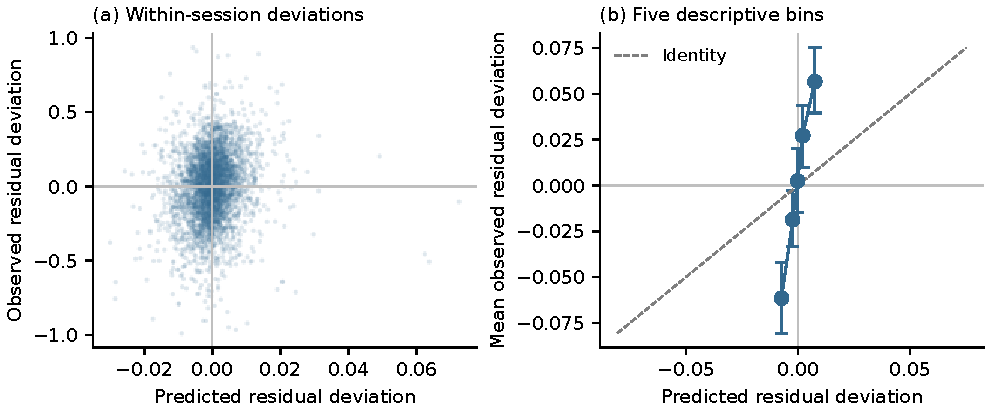
\includegraphics[width=.95\textwidth]{../../outputs/forecasting/residual_prediction_diagnostic_h5.pdf}
\caption{Residual-target score-only GRU at horizon 5. Session means are
subtracted from predicted and observed residuals for this retrospective
display, not supplied to the forecaster. (a) All 3,780 held-out pairs.
(b) Five pooled predicted-deviation quantile bins; bin means give subjects
equal weight and bars show unadjusted descriptive 95\% subject-bootstrap
intervals. Bins and centring are display diagnostics, not training decisions.
The identity line indicates matching magnitudes.}
\label{fig:supp_residual_diagnostic}
\end{figure}

\clearpage
\begin{table}[!ht]
\centering\small
\setlength{\tabcolsep}{5pt}
\caption{Residual-target GRU associations with unadjusted descriptive 95\% subject-bootstrap intervals. SD ratio averages within-session predicted/observed residual SDs within subjects and then across subjects; it describes variation, not forecast calibration.}
\label{tab:supp_residual_gru_intervals}
\begin{tabular}{lrrrr}
\toprule
Model & $h$ & Pearson $r$ & 95\% interval & SD ratio \\
\midrule
GRU EEG & 5 & +0.173 & [+0.151, +0.196] & 0.121 \\
GRU EEG & 10 & +0.161 & [+0.122, +0.198] & 0.141 \\
GRU EEG & 15 & +0.138 & [+0.089, +0.186] & 0.181 \\
GRU EEG & 20 & +0.112 & [+0.082, +0.143] & 0.175 \\
GRU EEG & 25 & +0.049 & [-0.003, +0.098] & 0.166 \\
GRU hybrid & 5 & +0.197 & [+0.176, +0.217] & 0.126 \\
GRU hybrid & 10 & +0.179 & [+0.137, +0.222] & 0.150 \\
GRU hybrid & 15 & +0.162 & [+0.119, +0.207] & 0.169 \\
GRU hybrid & 20 & +0.136 & [+0.097, +0.172] & 0.164 \\
GRU hybrid & 25 & +0.069 & [+0.002, +0.133] & 0.160 \\
GRU score & 5 & +0.182 & [+0.148, +0.215] & 0.023 \\
GRU score & 10 & +0.112 & [+0.067, +0.156] & 0.042 \\
GRU score & 15 & +0.095 & [+0.048, +0.143] & 0.026 \\
GRU score & 20 & +0.136 & [+0.082, +0.190] & 0.029 \\
GRU score & 25 & +0.091 & [+0.045, +0.133] & 0.045 \\
\bottomrule\end{tabular}\end{table}


Intervals use 10,000 subject bootstrap resamples and seed 20261011,
condition on saved fits, and omit refitting/model-selection uncertainty.
They are unadjusted, descriptive intervals; no residual-correlation
significance tests or equivalence claims are added. Shared LOSO training,
short session series, and overlapping windows limit their interpretation.
Full-session centring can affect finite-series lag correlations; the original
centred-lag diagnostic does not prove an absence of temporal structure.

Small positive residual associations coexist with limited MAE gains.
At horizon 5, the residual score-only GRU's mean within-session correlation
is 0.182 (95\% interval $[0.148,0.215]$), but its predicted/observed residual
SD ratio averages only 0.023. EEG and hybrid residual GRUs give correlations
0.173 and 0.197 and SD ratios 0.121 and 0.126, respectively.
The small SD ratio describes compressed predictive variation; it does not alone
establish miscalibration, since conditional-mean forecasts can vary less than
noisy observations. These associations concern direction and covariation; they do not establish
accurate forecast magnitudes, behavioural meaning, or an MAE advantage.
Subtracting the recent mean defines the target; it does not isolate a purely
physiological dynamic component. Both fitted views, all session metrics,
subject aggregates, eligibility counts, and the figure's points/bins are supplied.

\clearpage
\section{Training-subject-fitted calibration correction}\label{sec:supp_calibration_correction}

The strong calibration/online session-mean association and systematic offset
motivate one further post-hoc baseline:
\begin{equation}
\hat s_{b+h}=a_{-u}+c_{-u}\bar s^{\mathrm{avatar}}_{u,j,\mathrm{cal}}.
\end{equation}
For fold $u$, ordinary least squares maps avatar-calibration means to full
50-block online-session means using the other 14 subjects' 98 sessions.
Sessions have equal weight (seven per subject). Only training subjects' online
outcomes enter fitting. Prediction uses the held-out session's calibration
mean, available before online operation; coefficients are shared across
horizons and anchors. No blend, clipping, tuning, or alternative correction
is selected. The supplied specification,
\path{docs/paper_revision/calibration_correction_protocol.md}, was written before
evaluating this correction, after reviewing earlier diagnostics.

\begin{table}[!ht]
\centering\small
\setlength{\tabcolsep}{5pt}
\caption{Post-hoc training-subject-fitted affine calibration correction. MAE gives subjects equal weight. Context and expanding means use observed online history; the correction uses only the held-out session's calibration mean.}
\label{tab:supp_calibration_correction}
\begin{tabular}{lrrr}
\toprule
Horizon & Context mean & Expanding mean & Corrected calibration \\
\midrule
1 & 0.1721 & 0.1691 & 0.1946 \\
2 & 0.1724 & 0.1690 & 0.1940 \\
3 & 0.1736 & 0.1697 & 0.1939 \\
4 & 0.1741 & 0.1700 & 0.1938 \\
5 & 0.1746 & 0.1701 & 0.1933 \\
10 & 0.1741 & 0.1710 & 0.1932 \\
15 & 0.1767 & 0.1720 & 0.1925 \\
20 & 0.1773 & 0.1723 & 0.1919 \\
25 & 0.1752 & 0.1739 & 0.1943 \\
\bottomrule\end{tabular}\end{table}


Correction substantially improves the uncorrected calibration forecast:
at horizon 5, MAE falls from 0.4523 to 0.1933, a 57.3\% reduction.
Across horizons, corrected MAE is 0.1919--0.1946; both the recent and expanding
online means nevertheless have lower MAE at every horizon after correction.
The largest adjusted $p$ is 0.0215 versus the context mean and 0.0137 versus
the expanding mean. Fold slopes range from 0.8524 to 0.8863 and intercepts
from $-0.1849$ to $-0.1075$. Calibration therefore contains useful level
information after correcting bias, but this mapping does not match estimates
based on observed online history. The comparison concerns these predictors,
not the value of calibration information in all possible models.

\begin{table}[!ht]
\centering\small
\setlength{\tabcolsep}{5pt}
\caption{Post-hoc corrected-calibration contrasts (correction minus comparator). Intervals are unadjusted descriptive 95\% subject bootstraps. $p_{18}$ corrects all 18 correction tests in a family separate from Table S15.}
\label{tab:supp_calibration_correction_pairs}
\begin{tabular}{lrrrr}
\toprule
Comparator & $h$ & $\Delta$ MAE & 95\% interval & $p_{18}$ \\
\midrule
Context mean & 1 & +0.02252 & [+0.01240, +0.03333] & 0.0116 \\
Expanding mean & 1 & +0.02549 & [+0.01572, +0.03617] & 0.0022 \\
Context mean & 2 & +0.02158 & [+0.01127, +0.03254] & 0.0210 \\
Expanding mean & 2 & +0.02502 & [+0.01517, +0.03582] & 0.0049 \\
Context mean & 3 & +0.02029 & [+0.01030, +0.03097] & 0.0210 \\
Expanding mean & 3 & +0.02416 & [+0.01433, +0.03497] & 0.0049 \\
Context mean & 4 & +0.01972 & [+0.00958, +0.03057] & 0.0210 \\
Expanding mean & 4 & +0.02379 & [+0.01398, +0.03465] & 0.0056 \\
Context mean & 5 & +0.01872 & [+0.00848, +0.02966] & 0.0210 \\
Expanding mean & 5 & +0.02315 & [+0.01355, +0.03380] & 0.0056 \\
Context mean & 10 & +0.01911 & [+0.00962, +0.02993] & 0.0210 \\
Expanding mean & 10 & +0.02221 & [+0.01333, +0.03248] & 0.0031 \\
Context mean & 15 & +0.01574 & [+0.00653, +0.02632] & 0.0210 \\
Expanding mean & 15 & +0.02043 & [+0.01159, +0.03077] & 0.0049 \\
Context mean & 20 & +0.01463 & [+0.00443, +0.02565] & 0.0215 \\
Expanding mean & 20 & +0.01960 & [+0.01010, +0.03038] & 0.0137 \\
Context mean & 25 & +0.01905 & [+0.00889, +0.03001] & 0.0210 \\
Expanding mean & 25 & +0.02034 & [+0.01127, +0.03037] & 0.0067 \\
\bottomrule\end{tabular}\end{table}


The 18 correction-versus-online-mean contrasts use identical examples and
two-sided subject-paired Wilcoxon tests with Pratt zero handling. One all-18
Holm family is separate from Table S15 and historical families. Descriptive
intervals use 10,000 subject resamples and seed 20261011, conditional on fits;
shared LOSO training and omitted refitting uncertainty remain limitations.
The same participants are reused, without independent confirmation. A blend
and point-loss GRU are deferred. Saved fold parameters, training-subject lists,
29,820 predictions, 135 subject MAEs, nine summaries, and 18 tests are supplied.

\clearpage
\section{Availability, provenance, and reproduction}

The local package is named \texttt{forecastability-limits-proxy-bciaut-p300}.
The project repository is:\par
\repositorylink\par
The package includes supplementary sources and its PDF, derived results,
relevant pipeline code, \path{pyproject.toml}, \path{uv.lock}, and a SHA-256
source manifest. The main manuscript is maintained separately.
Raw EEG and third-party research-paper PDFs are not redistributed.

\path{pipeline/build_paper_supplement.py} reads saved inputs, verifies
original paired means/differences, reproduces pooled
ranking, and regenerates diagnostic results, tables, and the paired-difference
figure. It fits only the affine calibration correction and preserves historical
result files. An optional external manuscript argument checks all 80 original
main-table MAEs and the five expanding-mean values added to Table I.
It also verifies the 40 short-horizon MAE entries, their 600 subject metrics,
and all 32 new paired comparisons, and regenerates Tables S10--S13.
\path{pipeline/verify_paper_inference.py} separately checks the original
340 tests and Holm corrections.
\path{pipeline/build_paper_feedback_addendum.py} reproduces the two additional
fixed baselines, the 18 new paired tests, calibration-mean checks, continuous
residual diagnostics, Tables S14--S19, and Figure S1 from saved artifacts,
and fits the training-only affine calibration correction with 18 further tests.
The supplement builder invokes it automatically; no original classical or GRU
model is retrained. Its independent verifier reconstructs all 15 calibration
fits via centered covariance and audits the new predictions and inference.

The manifest hashes source/input files, records package versions and bootstrap
settings, identifies corrected ranking inputs, and lists excluded historical
ranking files. Outputs under
\path{data/forecasting/review_revision/supplementary/} include:
\begin{itemize}
\item \path{full_model_summary.csv}: 170 model/view/horizon summaries.
\item \path{subject_metrics.csv}: 2,550 subject-fold metric rows.
\item \path{paired_mae_differences.csv}: 2,400 paired subject differences.
\item \path{original_tested_contrasts.csv}: 340 original paired tests.
\item \path{contrast_templates.csv}: 17 original contrast templates.
\item \path{contrast_definitions.csv}: 23 instantiated ordered model pairs.
\item \path{selected_classical_comparators.csv}: 20 comparator selections.
\item \path{ranking_session_metrics.csv}: session eligibility and ranking metrics.
\item \path{ranking_subject_metrics.csv}: both subject ranking aggregations.
\item \path{ranking_summary.csv}: ranking summaries and descriptive intervals.
\item \path{robustness_summary.csv}: 90 GRU/view/horizon/protocol summaries.
\item \path{probabilistic_summary.csv}: Gaussian NLL, coverage, and interval width.
\item \path{variance_components.csv}: the constructed score's variance partition.
\item \path{score_diagnostics.json}: score partition and context correlations.
\item \path{snapshot_manifest.json}: source/input hashes and analysis provenance.
\item \path{short_horizon_summary.csv}: 40 additional model/view/horizon summaries.
\item \path{short_horizon_subject_metrics.csv}: 600 short-horizon subject metrics.
\item \path{short_horizon_paired_mae_stats.csv}: 32 new tests, effects, intervals,
and both Holm corrections.
\item \path{additional_baseline_predictions.csv}: all 29,820 example keys,
observed targets, and the three fixed predictions.
\item \path{additional_baseline_subject_metrics.csv}: 405 subject MAEs.
\item \path{additional_baseline_summary.csv}: 27 baseline/horizon summaries.
\item \path{additional_baseline_paired_stats.csv}: 18 post-hoc paired tests.
\item \path{calibration_correction_fold_parameters.csv}: 15 training-only affine fits.
\item \path{calibration_correction_predictions.csv}: 29,820 held-out forecasts.
\item \path{calibration_correction_subject_metrics.csv}: 135 subject MAEs.
\item \path{calibration_correction_summary.csv}: nine equal-subject summaries.
\item \path{calibration_correction_paired_stats.csv}: 18 further post-hoc tests.
\item \path{calibration_mean_session_diagnostics.csv}: per-session means and bias.
\item \path{calibration_mean_diagnostics.json}: signs, distribution and correlations.
\item \path{residual_association_session_metrics.csv}: within-session associations.
\item \path{residual_association_subject_metrics.csv}: subject aggregates.
\item \path{residual_association_summary.csv}: uncertainty, variation and eligibility.
\item \path{residual_diagnostic_h5_points.csv}: Figure S1's held-out pairs.
\item \path{residual_diagnostic_h5_bins.csv}: Figure S1's bin means and intervals.
\item \path{additional_analysis_provenance.json}: analysis definitions,
hashes and verification settings.
\item \path{additional_analysis_verification.json}: independent audit results.
\end{itemize}

The completed short-horizon experiment is stored separately under
\path{data/forecasting/review_revision/short_horizons/}, including predictions,
selected settings, the locked protocol, source/input hashes, reference checks,
and an independent exhaustive signed-rank audit. All 161,700 predictions
reproduce their 600 subject MAEs. The inference audit reproduces all 32 raw
p-values, both Holm correction schemes, and all bootstrap intervals.
\path{pipeline/exp41_paper_short_horizons.py} refits this analysis from the
frozen Step 4/5 artifacts. It preserves completed experiment checkpoints;
after source or manuscript revisions, use a new output directory.

Large prediction CSVs are supplied as lossless gzip archives. Analysis tools
read them directly, preferring an uncompressed CSV if one has been regenerated.
The portable release inventory and compressed/uncompressed hashes are in
\path{docs/paper_revision/release_manifest.json}; original thesis manifests
are retained separately as historical provenance. The reproduction guide
documents rebuilding the analyses without the private manuscript source.

\bibliographystyle{supplementary_generated/IEEEtran}
\bibliography{supplementary_generated/references}
\end{document}
